% \documentclass[12pt, twoside]{book}
\documentclass[12pt, oneside]{book}  % jednostranna tlac

%spravne nastavenie okrajov
\usepackage[a4paper,top=2.5cm,bottom=2.5cm,left=3.5cm,right=2cm]{geometry}
%zapnutie fontov pre UTF8 kodovanie
\usepackage[utf8]{inputenc}
\usepackage[T1]{fontenc}
\usepackage{lmodern}
\usepackage{amsmath}
\usepackage{enumitem}
\usepackage{array}
\usepackage{xcolor}

%zapnutie slovenskeho delenia slov
%a automatickych nadpisov ako Obsah, Obrázok a pod. v slovencine
%\usepackage[slovak]{babel} % vypnite pre prace v anglictine!

%nastavenie riadkovania podla smernice
\linespread{1.25} % hodnota 1.25 by mala zodpovedat 1.5 riadkovaniu

% balicek na vkladanie zdrojoveho kodu
\usepackage{listings}
% ukazky kodu su cislovane ako Listing 1,2,...
% tu je Listing zmenene na Algoritmus 1,2,...
\renewcommand{\lstlistingname}{Listing}
% nastavenia balicka listings

\lstdefinelanguage{JavaScript}{
  keywords={break, case, catch, continue, debugger, default, delete, do, else, finally, for, function, if, in, instanceof, new, return, switch, this, throw, try, typeof, var, void, while, with},
  morecomment=[l]{//},
  morecomment=[s]{/*}{*/},
  morestring=[b]',
  morestring=[b]",
  sensitive=true
}

\lstset{
  language=JavaScript,
  frame=none,
  backgroundcolor=\color{gray!7},
  basicstyle=\small\ttfamily,
  showstringspaces=false,
  showspaces=false,
  numbers=left,
  numberstyle=\small\ttfamily\color{gray},
  numbersep=9pt,
  tabsize=2,
  breaklines=true,
  showtabs=false,
  captionpos=b,
  xleftmargin=15pt,
  xrightmargin=15pt
}

% balicek na vkladanie obrazkov
\usepackage{graphicx}
% balicek na vkladanie celych pdf dokumentov, tu zadanie
\usepackage{pdfpages}
% balicek na spravne formatovanie URL
\usepackage{url}
% balicek na hyperlinky v ramci dokumentu
% zrusime farebne ramiky okolo liniek aby pdf
% vyzeralo rovnako ako tlacena verzia
\usepackage[hidelinks,breaklinks]{hyperref}

% -------------------
% --- Definicia zakladnych pojmov
% --- Vyplnte podla vasho zadania, rok ma byt rok odovzdania
% -------------------
\def\mfrok{2025}
\def\mftitle{Analysis, Design and Implementation of Micro-frontend Architecture}
\def\mftyp{Bachelor Thesis}
\def\mfauthor{Bc. Pavol Repiský}
\def\mfskolitel{RNDr. Ľubor Šešera, PhD.}

%ak mate konzultanta, odkomentujte aj jeho meno na titulnom liste
\def\mfkonzultant{Ing. Juraj Marák}  

\def\mfmiestocas{Bratislava, \mfrok}
\def\mfuniverzita{COMENIUS UNIVERSITY IN BRATISLAVA}
\def\mffakulta{FACULTY OF MATHEMATICS PHYSICS AND INFORMATICS}
\def\mftypprace{Diploma thesis}

\def\mfodbor{Computer Science}
\def\program{Applied Computer Science}

% Ak je školiteľ z FMFI, uvádzate katedru školiteľa, zrejme by mala byť aj na zadaní z AIS2
\def\mfpracovisko{Department of Computer Science}

\begin{document}     
\frontmatter
\pagestyle{empty}

\noindent
\begin{minipage}{\textwidth}
    \begin{center}
      \textbf{\mfuniverzita\\
      \mffakulta}
    \end{center}
\end{minipage}

\vfill
\begin{figure}[!hbt]
	\begin{center}
		
\includegraphics[width=0.4\textwidth]{images/FMFI_logo_BP.png}
		\label{img:logo}
	\end{center}
\end{figure}
\begin{center}
		\textbf{\MakeUppercase{\Large\mftitle}}\\
    \mftypprace
\end{center}
\vfill
\mfrok \hfill
\mfauthor
%\eject 
\cleardoublepage
% --- koniec obalky ----


% -------------------
% --- Titulný list
% -------------------
\thispagestyle{empty}
\noindent
\begin{minipage}{\textwidth}
    \begin{center}
      \textbf{\mfuniverzita\\
      \mffakulta}
    \end{center}
\end{minipage}

\vfill
\begin{figure}[!hbt]
    \begin{center}
        
\includegraphics[width=0.4\textwidth]{images/FMFI_logo_BP.png}
        \label{img:logo_dark}
    \end{center}
\end{figure}

\begin{center}
	\textbf{\MakeUppercase{\Large\mftitle}}\\
	\mftypprace
\end{center}
\vfill


\begin{tabular}{l l}
Study program: & \program \\
Branch of study: & \mfodbor \\
Department: & \mfpracovisko \\
Supervisor: & \mfskolitel \\
Consultant: & \mfkonzultant \\
\end{tabular}

\vfill
\noindent
\mfmiestocas \hfill
\mfauthor
%\eject 
\cleardoublepage
% --- Koniec titulnej strany



% -------------------
% --- Zadanie z AIS
% -------------------
% v tlačenej verzii s podpismi zainteresovaných osôb.
% v elektronickej verzii sa zverejňuje zadanie bez podpisov
% v pracach v anglictine anglicke aj slovenske zadanie

\newpage
\setcounter{page}{2}
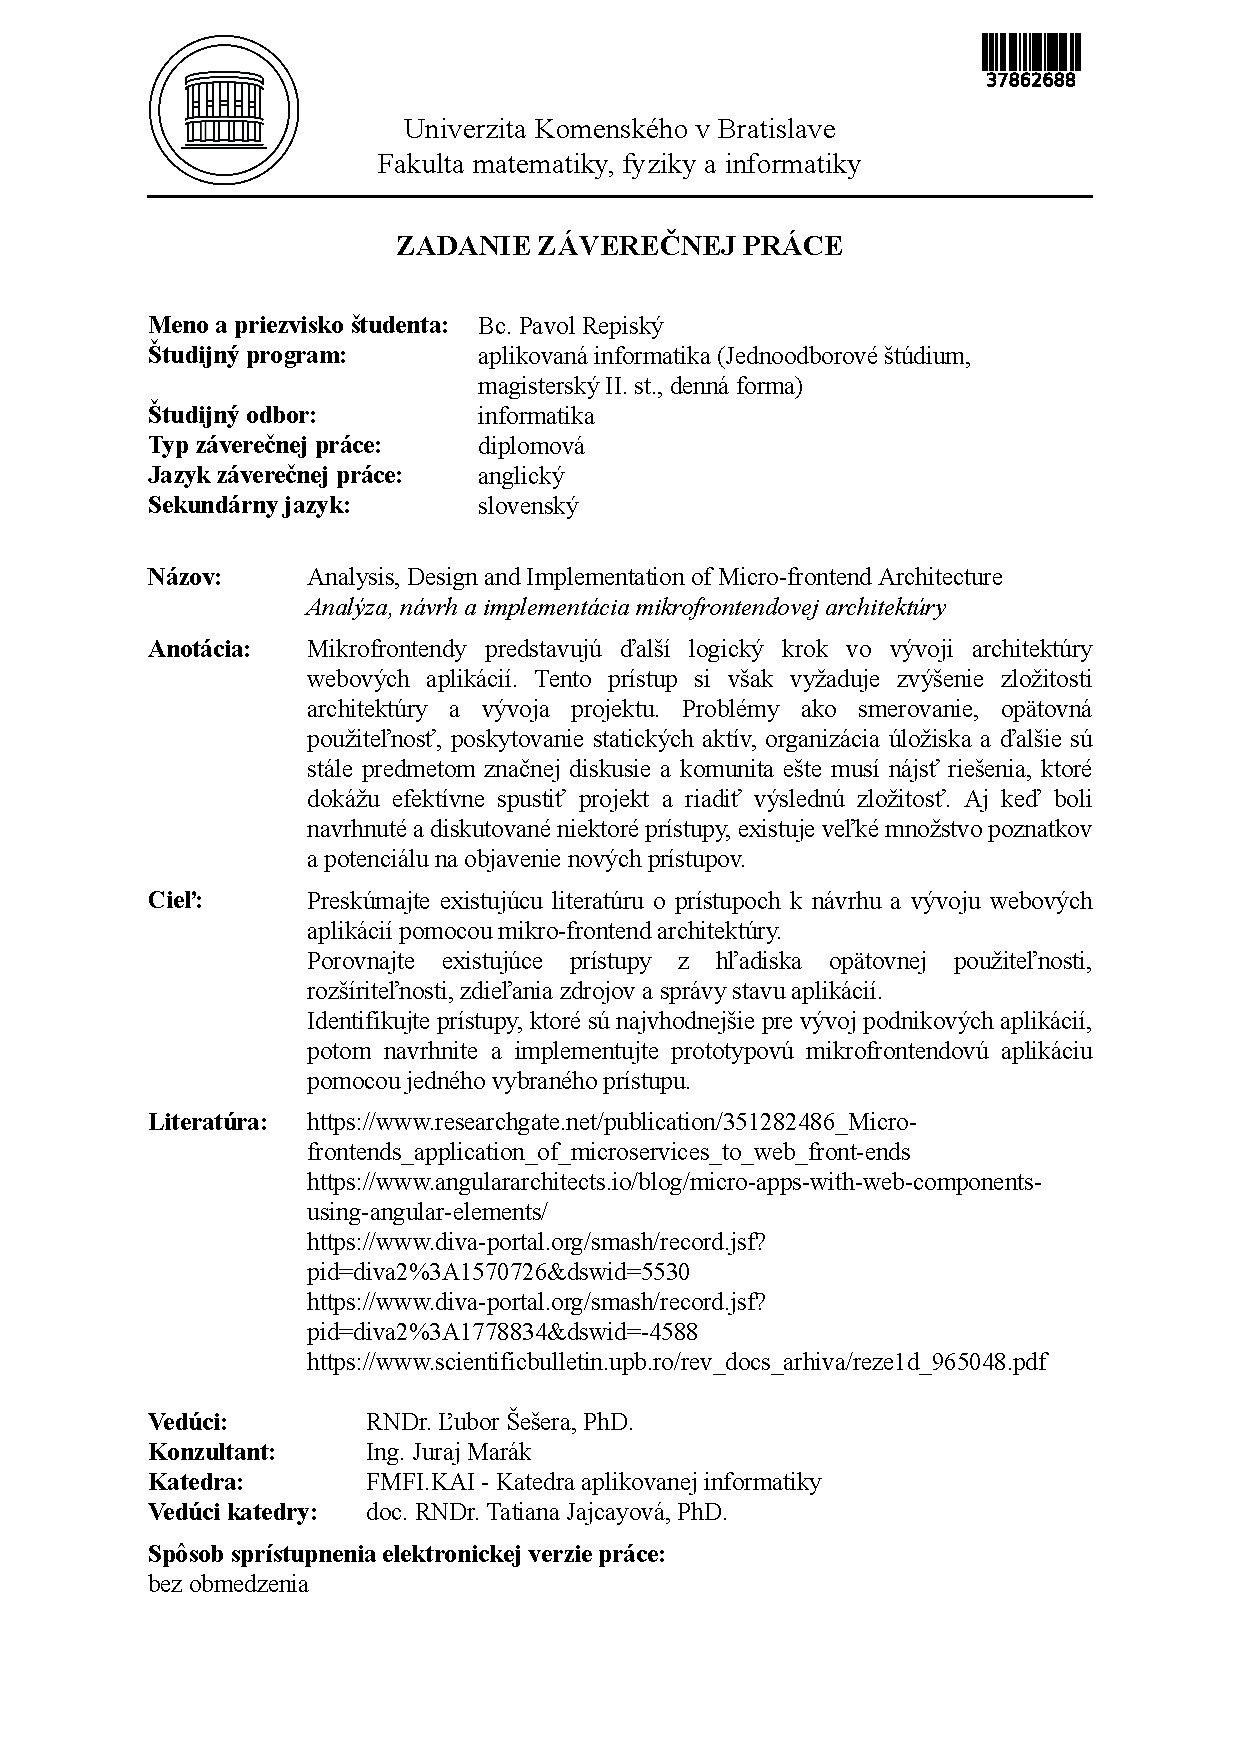
\includepdf[pages=-]{images/zadanie.pdf}

\includepdf[pages=-]{images/zadanie-en.pdf}
% --- Koniec zadania


% -------------------
%   Declaration
% -------------------
\newpage
\thispagestyle{empty}
\chapter*{Declaration}\label{chap:declaration}
I hereby declare that I have completed this thesis independently, without any assistance from third parties, and without using any sources or aids other than those explicitly cited.

\vfill

\hfill \makebox[5cm]{\dotfill} \newline
Bratislava, \mfrok \hfill \mfauthor \hspace{0.8cm}
% --- Koniec vyhlásenia

% -------------------
%   Poďakovanie - nepovinné
% -------------------
\newpage
\thispagestyle{empty}
\chapter*{Acknowledgement}\label{chap:thank_you}
I want to thank RNDr. Ľubor Šešera, PhD., for his supervision, willingness, and valuable advice. I am also very grateful to Ing. Juraj Marák for his patience, guidance, and the time he devoted to me during the preparation of my thesis.

\vfill\eject 
% --- Koniec poďakovania

% -------------------
%   Abstrakt - Slovensky
% -------------------
\newpage 
\thispagestyle{empty}
\chapter*{Abstrakt}\label{chap:abstract_sk}
Táto práca sa zaoberá mikrofrontendmi vo viacvrstvových podnikových webových aplikáciách. V prvých kapitolách poskytuje prehľad súčasnej literatúry o architektúre mikrofrontendov a porovnáva sedem najčastejšie používaných prístupov k mikrofrontendom z viacerých hľadísk, ako sú rozšíriteľnosť, znovupoužiteľnosť, jednoduchosť, výkonosť, zdieľanie zdrojov, používateľská skúsenosť vývojára a samotné využitie. V závere prehľadovej časti identikujeme tri prístupy, ktoré sú vhodné pre podnikové aplikácie. Z týchto prístupov sme vybrali prístup, ktorý považujeme za najperspektívnejší, konkrétne Web Components, pre implementáciu prototypovej aplikácie. Vybraná aplikácia predstavuje zjednodušenú verziu nástroja na správu projektov. Práca opisuje návrh a implementáciu tejto prototypovej aplikácie. Na implementáciu sme zvolili framework Angular \cite{Angular}, ktorý patrí medzi najpoužívanejšie frameworky na vývoj moderných frontendov v podnikových webových aplikáciách. V závere práce vyhodnocujeme implementovanú aplikáciu z viacerých hľadísk, vrátane rozšíriteľnosti, znovu-použiteľnosti, zdieľania zdrojov a správy aplikačného stavu.

\paragraph*{Kľúčové slová:} Microfrontends, Web Components, architektúry webových aplikácií, Angular
% --- Koniec Abstrakt - Slovensky


% -------------------
% --- Abstrakt - Anglicky 
% -------------------
\newpage 
\thispagestyle{empty}
\chapter*{Abstract}\label{chap:abstract_en}
This thesis addresses microfrontends in multi-tier enterprise web applications. First, it reviews the current literature on microfrontend architecture and compares the seven most commonly used approaches to microfrontends from several aspects, such as extensibility, reusability, simplicity, performance, resource sharing, developer experience, and usage. It identifies three approaches that are suitable for enterprise applications. From these, it selects the approach, we consider to be the most promising, namely, Web Components, for the implementation of a prototypical application. The chosen application is a simplified version of a project management tool. The thesis describes the design and implementation of this prototypical application. For the implementation, we chose the Angular \cite{Angular} framework, which is one of the most widely used frameworks for developing modern frontends in enterprise web applications. Finally, we evaluated the implemented application from several aspects, including extensibility, reusability, resource sharing, and application state management.

\paragraph*{Keywords:} Microfrontends, Web Components, web application architectures, Angular
% --- Koniec Abstrakt - Anglicky

% -------------------
% --- Predhovor - v informatike sa zvacsa nepouziva
% -------------------
%\newpage 
%
%
%\chapter*{Preface} %
%
%Predhovor je všeobecná informácia o práci, obsahuje hlavnú charakteristiku práce 
%a okolnosti jej vzniku. Autor zdôvodní výber témy, stručne informuje o cieľoch 
%a význame práce, spomenie domáci a zahraničný kontext, komu je práca určená, 
%použité metódy, stav poznania; autor stručne charakterizuje svoj prístup a svoje
%hľadisko. 
%
% --- Koniec Predhovor


% -------------------
% --- Obsah
% -------------------

\newpage 

\tableofcontents

% ---  Koniec Obsahu

% -------------------
% --- Zoznamy tabuliek, obrázkov - nepovinne
% -------------------

\newpage 

\listoffigures
\listoftables
\lstlistoflistings

% ---  Koniec Zoznamov

\mainmatter
\pagestyle{headings}

\input chapters/introduction/Introduction.tex 
\input chapters/microservices_and_microfrontends/MicroservicesAndMicrofrontends.tex
\input chapters/microfrontends_in_detail/MicrofrontendsInDetail.tex
\input chapters/design/Design.tex
\input chapters/implementation/Implementation.tex
\input chapters/evaluation_results/EvaluationResults.tex
\input chapters/conclusion/Conclusion.tex

% -------------------
% --- Bibliografia
% -------------------


\newpage	

\backmatter

\thispagestyle{empty}
\clearpage

\bibliographystyle{ieeetr}
\bibliography{literatura} 

%---koniec Referencii

% -------------------
%--- Prilohy---
% -------------------

%Nepovinná časť prílohy obsahuje materiály, ktoré neboli zaradené priamo  do textu. Každá príloha sa začína na novej strane.
%Zoznam príloh je súčasťou obsahu.
%
%\input appendixA.tex
%\input appendixB.tex

\end{document}






